% Name: Bipartite graph with a matching
% Description: Workers and the jobs they can do, with a perfect matching drawn in green.
% Tags: bipartite graph, matching, assignment

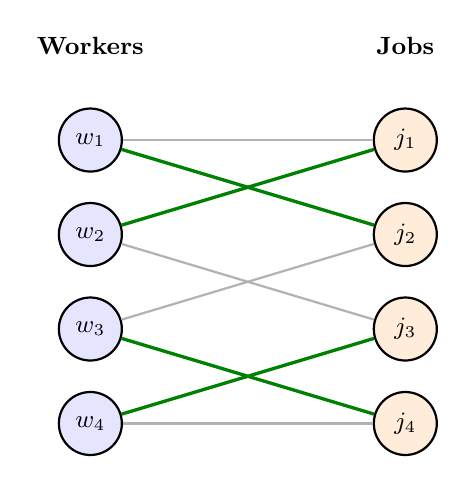
\begin{tikzpicture}[
  worker/.style={circle, draw, thick, fill=blue!10, minimum size=8mm, font=\small},
  job/.style={circle, draw, thick, fill=orange!15, minimum size=8mm, font=\small},
]
  \foreach \i in {1,...,4} {
    \node[worker] (w\i) at (0,-1.2*\i) {$w_{\i}$};
    \node[job] (j\i) at (4,-1.2*\i) {$j_{\i}$};
  }
  \node[font=\small\bfseries] at (0,0) {Workers};
  \node[font=\small\bfseries] at (4,0) {Jobs};

  \foreach \a/\b in {1/1, 2/3, 3/2, 4/4}
    \draw[thick, gray!60] (w\a) -- (j\b);
  \foreach \a/\b in {1/2, 2/1, 3/4, 4/3}
    \draw[very thick, green!50!black] (w\a) -- (j\b);
\end{tikzpicture}
